\documentclass{article}

\usepackage{ewrl_2026}

\usepackage[utf8]{inputenc}
\usepackage[T1]{fontenc}
\usepackage{hyperref}
\usepackage{url}
\usepackage{booktabs}
\usepackage{amsfonts}
\usepackage{amsmath, amssymb}
\usepackage{nicefrac}
\usepackage{microtype}
\usepackage{xcolor}
\usepackage{graphicx}
\usepackage{subcaption}
\usepackage{algorithm}
\usepackage{algpseudocode}
\usepackage{tikz}
\usetikzlibrary{arrows.meta, positioning, shapes.geometric, fit, backgrounds}

\newcommand{\physigym}{\textsc{PhysiGym}}
\newcommand{\physicell}{\textsc{PhysiCell}}
\newcommand{\Itwo}{\texttt{img\_mc\_cells\_substrates}}
\newcommand{\Ione}{\texttt{img\_mc\_cells}}
\newcommand{\Sone}{\texttt{scalars\_cells}}
\newcommand{\Stwo}{\texttt{scalars\_cells\_substrates}}
\newcommand{\Sthree}{\texttt{spatial\_scalars\_cells}}
\newcommand{\Sfive}{\texttt{spatial\_scalars\_cells\_spatial\_substrates}}

% ─────────────────────────────────────────────────────────────────────────────

\title{\physigym{}: Bridging Agent-Based Biological Simulation and Reinforcement
  Learning — A State-Space Study on Tumor Microenvironment Control}

\author{%
  Alexandre Bertin$^{1,2,5,\dagger}$ \quad
  Elmar Bucher$^{3,\dagger}$ \quad
  Owen Griere$^{2,5}$ \quad
  Marcelo Hurtado$^{2,5}$ \\
  Heber Rocha$^{3}$ \quad
  Randy Heiland$^{3}$ \quad
  Paul Macklin$^{3,\ddagger}$ \quad
  Vincent Fran\c{c}ois-Lavet$^{4,\ddagger}$ \\
  Emmanuel Rachelson$^{1,\ddagger}$ \quad
  Vera Pancaldi$^{2,5,\ddagger}$ \\[4pt]
  $^1$CRCT, Université de Toulouse, Inserm, CNRS, Université Toulouse III--Paul Sabatier, France \\
  $^2$ISAE-Supaéro, Toulouse, France \quad
  $^3$Dept.\ of Intelligent Systems Engineering, Indiana University, USA \\
  $^4$Dept.\ of Computer Science, VU Amsterdam, The Netherlands \quad
  $^5$Équipe Labellisée LIGUE Contre le Cancer, France \\[2pt]
  {\small $^\dagger$Equal first-author contribution. $^\ddagger$Equal senior-author contribution.}
}

\begin{document}

\maketitle

\begin{abstract}
This paper presents \physigym{}, a framework that integrates agent-based
biological simulation within standardised reinforcement learning environments.
By connecting the agent-based modelling framework \physicell{} with the
Gymnasium API, we provide a flexible tool for exploring RL strategies that
control \emph{in silico} biological processes.
We demonstrate \physigym{}'s potential through a case study on a simplified
tumor microenvironment (TME) toy model, in which a Soft Actor-Critic agent
learns targeted drug-delivery policies that steer the microenvironment toward an
anti-tumoral state and, in the best episodes, achieve tumor elimination.
We further use this case study to systematically compare six observation
spaces — from global cell counts to full multi-channel spatial images.
We find that spatially explicit image observations including substrate
concentration maps learn faster and generalize better than scalar summaries
(mean training return $+77.2$ vs.\ $+5.9$, mean held-out test return
$+56.5$ vs.\ $+17.6$), demonstrating that \physigym{}'s flexible state-space
interface directly impacts policy quality in spatially structured environments.
\physigym{} is open-source at \url{https://github.com/Dante-Berth/PhysiGym}.
\end{abstract}

% ─────────────────────────────────────────────────────────────────────────────
\section{Introduction}
% ─────────────────────────────────────────────────────────────────────────────

Biological systems are complex, dynamic, and often difficult to study in real
life.
In silico modeling aims to mimic these systems, providing a controlled
environment for exploring specific aspects of biological processes and testing
hypotheses.
In particular, agent-based models (ABMs) provide a powerful framework for
simulating biological systems where agents (e.g.\ cells) interact dynamically
based on predefined rules. These models are used in oncology and immunology to
study emerging behaviors in complex biological systems, with the potential to
propose novel therapeutic strategies~\citep{johnson2023digitize,
laubenbacher2024toward, rocha2024multiscale}.

Ordinary differential equations (ODEs) and agent-based models (ABMs) are widely
used to simulate the tumor microenvironment (TME). ODEs provide compact
system-level descriptions, while ABMs capture spatial and cellular
heterogeneity at higher computational cost. For dynamic treatment regimes
(DTRs)~\citep{gray1982arac}, however, simulation alone is insufficient:
designing adaptive, sequential interventions requires a control framework.
Reinforcement learning (RL), where an RL agent learns policies through
interaction with an environment, offers such a framework~\citep{barto1989learning}.
By modeling treatment regimes as a sequence of decisions, RL enables adaptive
control of biological simulations~\citep{chakraborty2014dynamic}. For efficient
experimentation and policy learning, RL further requires a standardized
interface. To address this, we introduce \physigym{}, an interface that connects
\physicell{}~\citep{ghaffarizadeh2018physicell}, an ABM framework for
multicellular simulations of tissues or cell cultures (tumor microenvironment,
other disease tissues, or bacteria colonies), with
Gymnasium~\citep{towers2024gymnasium}, a widely adopted RL application
programming interface (API).
\physicell{} enables flexible multiscale modeling of biological systems, coupled
with a sophisticated underlying physics simulator (the BioFVM diffusion
transport solver~\citep{ghaffarizadeh2016biofvm}), while Gymnasium provides a
structured framework for training and evaluating RL policies.

The first implementation of RL on an ABM framework based on BioFVM was proposed
by \citet{zade2020reinforcement}, which applied Q-learning~\citep{watkins1992q}
to optimize Temozolomide treatment regimes for patients with glioblastoma
multiforme, a highly specific problem.
More recently, \citet{aif2025failing} used \physicell{} as a complex
(high-fidelity) simulation environment for tumor growth, combined with a simple
(low-fidelity) RL training environment of coupled ordinary differential
equations (ODE) to learn treatment strategies for solid tumors.

\physigym{} bridges \physicell{} and Gymnasium to provide a reproducible and
scalable framework for integrating agent-based simulations of biological systems
with RL strategies. In the following, we present \physigym{}'s motivation and
design, demonstrating how it directly connects ABMs and RL to control complex
biological systems. In particular, we focus on the tumor microenvironment, a
biological system made up of cancer cells and surrounding immune and stromal
cells that engage in complex interactions and cross-talks, which is proven to be
crucial for an effective response to immunotherapy, an important therapeutic
approach in an increasing number of types of cancer.

To illustrate the framework, we build a simplified TME toy model and use it as
an end-to-end RL case study. This model also serves as a controlled testbed for
a practical question that arises in any spatially explicit biological
environment: among the many observation spaces \physigym{} can expose (scalars,
images, graphs), which ones help an RL agent learn an effective dynamic treatment
regime? We find that image-based observations that preserve the spatial layout of
cells and substrates outperform compact scalar summaries, both in cumulative
return and in generalization to held-out spatial configurations. This is an
application-level finding on a deliberately simplified model; the primary
contribution of this work is \physigym{} itself.

\paragraph{Contributions.}
(1)~\physigym{}: an open-source framework that bridges the \physicell{} ABM and
the Gymnasium RL API, turning any \physicell{} model into an RL environment with
minimal code changes.
(2)~A simplified TME toy model demonstrating an end-to-end RL case study in
which an agent learns a spatial drug-delivery policy that drives the
microenvironment toward an anti-tumoral state.
(3)~A systematic comparison of observation spaces on the toy model, showing
that spatially explicit (image) representations help RL learn and generalize
better than scalar summaries.

% ─────────────────────────────────────────────────────────────────────────────
\section{Methods}
% ─────────────────────────────────────────────────────────────────────────────
\subsection{\physigym{} design and implementation}
\label{sec:physigym}

\physicell{} is an ABM framework written in C++ and implemented to model
multicellular systems based on classical
mechanics~\citep{ghaffarizadeh2018physicell}. Cells are agents whose type
determines the specific rule set that governs their behavior and interactions
with the other agents and the environment. Substrates, like oxygen or cytokines,
can be modeled with the integrated BioFVM diffusive transport
solver~\citep{ghaffarizadeh2016biofvm}. In addition, intracellular models can be
integrated into cell agents~\citep{letort2018physiboss, ponce2023physiboss,
ruscone2024physiboss} to model specific behaviors based on each cell's
environment and gene regulatory networks. The extracellular matrix that
surrounds cells in tissues can also be modeled as a mesh of fibers for a more
realistic representation of the cells' physical environment~\citep{noel2024physimess}.
Together, these components enable the construction of ABMs that are spatially
explicit in two or three dimensions, off-lattice, center-based, and multiscale
in both space and time~\citep{metzcar2019review}.

RL is used to control discrete-time dynamical systems, which are typically
modeled as Markov Decision Processes
(MDPs)~\citep{bellman1957markovian, puterman2014markov}.
An MDP consists of four key elements:
\begin{enumerate}
    \item $S$ the state space, where $s\in S$ represents a state of the environment.
    \item $A$ the action space, where $a \in A$ represents an action applied to the environment (e.g.\ drug dose).
    \item $T$ the transition model, which defines how the environment evolves. Formally, the next state $s'$ is given by $s'\sim T(s,a)$ where $s$ is the current state and $a$ the action taken.
    \item $R$ the reward function, which evaluates whether an action was beneficial. Formally, $r = R(s,a)$ is the reward obtained by taking action $a$ in state $s$.
\end{enumerate}
The objective is to find the policy that maximizes the expected discounted
cumulative reward:
\[
  \underset{\pi\in\Pi}{\arg\max}\;
  \mathbb{E}\!\left[\sum_{t=0}^{\tau}\gamma^t r_t \mid s_0 = s,\,\pi\right],
\]
with $s_0$ the initial state, $\pi$ the policy, $\gamma$ the discount factor,
and $\tau$ the terminal timestep. In the RL community, the Gymnasium RL API is
widely used as a standard interface for MDPs, promoting code reuse and
modularity in RL algorithms and models.

\physigym{} bridges the gap between the \physicell{} ABM framework and the
Gymnasium RL API by extending the Python
interpreter~\citep{rossum1995extending, psf2024extending} with \physicell{}.
As a result, the ABM model is implemented in the same way as standard
\physicell{} models, using PhysiCell Studio~\citep{heiland2024physicellstudio}
and C++.

Any model implemented in \physicell{} can be converted into a \physigym{} model.
The interface between \physicell{} and Gymnasium is based on the \physicell{}
``user parameter'', ``custom data variable'', and ``custom data vectors'' data
constructs. Information, such as how much drug to apply to the domain, can only
be transferred over these variable types. The variables (for example, drug) can
easily be specified in PhysiCell Studio under the \texttt{User Params} and
\texttt{Cell Types / Custom Data} tab.
As a minimum requirement, the user must define the parameter $dt\_gym$, which
specifies the time interval at which interactions with the environment occur,
and the parameter $time$, a time tracker necessary to determine when to update
the environment. In addition, further parameters can be defined to control the
simulation, such as drug administration, which can serve as actions. Similarly,
other parameters can be designated to record specific quantities of interest,
which can then be used to construct the observations.

According to the transition function, for each episode (a complete sequence of
states, actions, and rewards from the start to the end of a trial), values from
these data constructs can be modified without having to recompile the source
code. There are three additional functions to define the state space (read
information from the simulation): \texttt{get\_cell} for cell position,
\texttt{get\_microenv} for substrate concentration, and \texttt{get\_graph} to
retrieve cell neighborhood information.

To extend the Python interpreter with \physicell{}, the main simulation loop,
written in C++, was split into three functions: \texttt{physicell\_start},
\texttt{physicell\_step}, and \texttt{physicell\_stop}, all of which can be
called from Python. The \texttt{physicell\_start} function initializes the
\physicell{} model, while \texttt{physicell\_stop} terminates the simulation.
The \texttt{physicell\_step} function is responsible for advancing the
environment by one time step based on the action taken by the reinforcement
learning agent. For most models, only \texttt{physicell\_step} needs to be
modified, e.g.\ to apply drugs to the ABM. Several additional C++ functions are
exposed in Python to facilitate data retrieval. These include functions to
obtain custom variables, vectors, \texttt{physicell\_get\_cell}, which provides
a matrix containing information about each cell, such as its type, coordinates,
and death status, and \texttt{physicell\_get\_microenv}. All exposed functions
are implemented in the C++ file \texttt{physicellmodule.cpp}.

By extending the necessary functions to obtain the desired control over the ABM
and modifying the \texttt{physicell\_step} function, users can compile the C++
code and integrate it with Python, particularly with the Gymnasium API. This
allows users to define \texttt{physicell\_model.py}, which implements a
Gymnasium-compatible environment. Specifically, \texttt{physicell\_model.py}
defines a child class of Gymnasium's environment class, inheriting from
\texttt{CorePhysiCellEnv}, which is specified in \texttt{physicell\_core.py}.
\texttt{CorePhysiCellEnv} is the main class that takes charge of the use of
\texttt{physicell\_start}, \texttt{physicell\_stop} and \texttt{physicell\_step}
which are model independent. This class handles interactions with the Gymnasium
framework. Users should modify \texttt{physicell\_model.py} to specify the
observation space, action spaces, and the reward, as well as any additional data
they wish to store.

\physigym{} was extensively tested for compiling and running on Linux, Windows
Subsystem for Linux, and macOS. Pytest unit tests are included in the code base,
and we use GitHub Actions for continuous integration. Installation and
troubleshooting how-tos, a modeling tutorial, an RL tutorial, and a reference
manual can be found at
\url{https://github.com/Dante-Berth/PhysiGym/tree/main/man}.

% ─────────────────────────────────────────────────────────────────────────────
\subsection{Implementation of a tumor microenvironment toy model}
\label{sec:model}
% ─────────────────────────────────────────────────────────────────────────────

We developed a simplified tumor microenvironment (TME) \emph{toy model} to
illustrate the potential uses of \physigym{}. The model is deliberately small
and computationally cheap so that we can train RL agents to convergence many
times over (across observation spaces and seeds), while still retaining the
spatial, multicellular, and chemically coupled structure that distinguishes
ABMs from ODE surrogates. It includes three cell types, five diffusible
substrates, and a set of simple agent-based rules. This toy model highlights how
the RL framework can control tumor progression by modulating the whole
microenvironment, rather than solely targeting cancer-cell killing.

\paragraph{Domain and dynamics.}
The model runs on a $63\!\times\!63\,\mu$m 2D domain (Table~\ref{tab:cells_subs}).
The RL gym step is $\Delta t = 15$\,min; episodes run up to $10{,}080$\,min
(7 simulated days), with early termination at tumor count $c_t \le 3$
(eradication) or $c_t > 256$ (uncontrolled growth).

\begin{table}[h]
  \caption{Cell types and substrates in the TME model.}
  \label{tab:cells_subs}
  \centering\small
  \begin{tabular}{llp{5.8cm}}
    \toprule
    \textbf{Entity} & \textbf{Key parameters} & \textbf{Role} \\
    \midrule
    Tumor       & prolif.\ $3\!\times\!10^{-4}$/min, immotile & Target population; secretes \texttt{tumor\_molecule} \\
    T-cell      & speed 0.1\,µm/min, immortal & Cytotoxic via cytokine; chemotaxis toward \texttt{anti\_tumoral} \\
    Macrophage  & speed 0.1\,µm/min & Dual M1/M2 phenotype; chemotaxis toward \texttt{tumor\_molecule} \\
    \midrule
    \texttt{anti\_tumoral\_factor} & diff.\ 3\,µm$^2$/min & M1 signal; attracts T-cells \\
    \texttt{pro\_tumoral\_factor}  & diff.\ 3\,µm$^2$/min & M2 signal; repels T-cells (indirect) \\
    \texttt{drug\_1}               & non-diffusing, decay 0.05/min & Agent-controlled; re-polarises macrophages \\
    \texttt{tumor\_molecule}       & diff.\ 2\,µm$^2$/min & Danger signal; drives M2 polarisation \\
    \texttt{cytokine}              & diff.\ 0.003\,µm$^2$/min & T-cell signal; induces tumor apoptosis \\
    \bottomrule
  \end{tabular}
\end{table}

Cell-hypothesis rules (CBHG v3.0, Hill functions) define two key feedback
loops: (i)~high \texttt{tumor\_molecule} tips macrophages toward M2
(increasing \texttt{pro\_tumoral}, decreasing \texttt{anti\_tumoral}, slowing
migration); (ii)~\texttt{drug\_1} reverses this to M1.
T-cells secrete cytokine, which drives tumor apoptosis (Hill $n=4$, half-max 0.5).
The drug therefore acts \emph{indirectly}: it re-polarises macrophages, which
restores anti-tumoral gradients, which guides T-cells to the tumor, which then
kill it via cytokine.
Figure~\ref{fig:signalling} shows this full signalling network.

\begin{figure}[t]
  \centering
  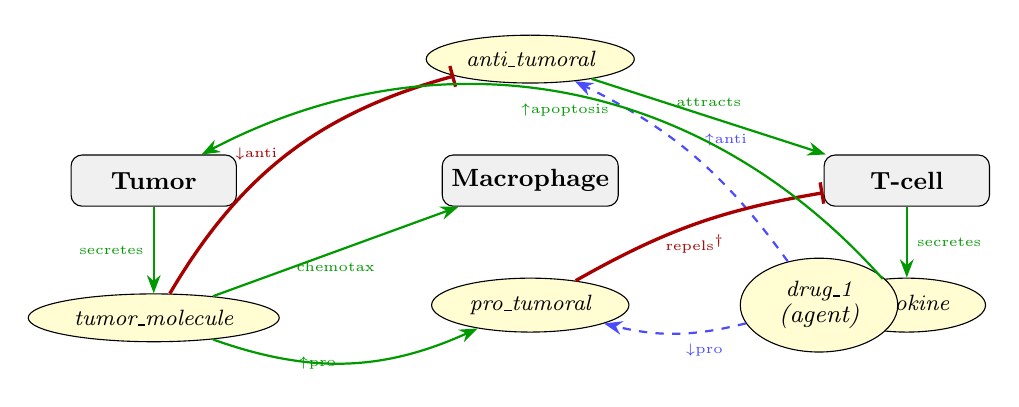
\begin{tikzpicture}[
      node distance = 1.3cm and 1.9cm,
      cell/.style  = {draw, rounded corners, fill=gray!12,
                      minimum width=2.1cm, minimum height=0.65cm,
                      font=\small\bfseries, align=center},
      sub/.style   = {draw, ellipse, fill=yellow!18,
                      minimum width=2.0cm, minimum height=0.52cm,
                      font=\footnotesize\itshape, align=center},
      act/.style   = {-Stealth, thick, green!60!black},
      inh/.style   = {-|, thick, red!65!black, line width=1.2pt},
      drug/.style  = {-Stealth, thick, blue!70, dashed},
    ]
    \node[cell]                       (tumor)  {Tumor};
    \node[sub, below=1.1cm of tumor]  (tmol)   {tumor\_molecule};
    \node[cell, right=2.6cm of tumor] (mac)    {Macrophage};
    \node[sub, below=0.9cm of mac]    (pro)    {pro\_tumoral};
    \node[sub, above=0.9cm of mac]    (anti)   {anti\_tumoral};
    \node[cell, right=2.6cm of mac]   (tcell)  {T-cell};
    \node[sub, below=0.9cm of tcell]  (cyto)   {cytokine};
    \node[sub, right=1.4cm of pro]    (drug)   {drug\_1\\\small(agent)};

    \draw[act] (tumor) -- node[left,  font=\tiny]{secretes}  (tmol);
    \draw[act] (tmol)  -- node[below, font=\tiny]{chemotax}  (mac);
    \draw[act] (tmol)  to[bend right=22] node[font=\tiny,left ]{$\uparrow$pro}  (pro);
    \draw[inh] (tmol)  to[bend left=22]  node[font=\tiny,left ]{$\downarrow$anti}(anti);
    \draw[drug](drug)  to[bend left=14]  node[font=\tiny,below right]{$\downarrow$pro} (pro);
    \draw[drug](drug)  to[bend right=14] node[font=\tiny,above right]{$\uparrow$anti}  (anti);
    \draw[act] (anti)  -- node[above, font=\tiny]{attracts}  (tcell);
    \draw[inh] (pro)   to[bend left=10]  node[font=\tiny,below]{repels$^\dagger$}(tcell);
    \draw[act] (tcell) -- node[right, font=\tiny]{secretes}  (cyto);
    \draw[act] (cyto)  to[bend right=38] node[font=\tiny,below]{$\uparrow$apoptosis}(tumor);
  \end{tikzpicture}
  \caption{TME signalling network.
    $\rightarrow$ = activation; $\dashv$ = inhibition (red);
    dashed blue = agent-controlled drug.
    $^\dagger$Repulsion of T-cells by \texttt{pro\_tumoral} is indirect:
    it displaces the \texttt{anti\_tumoral} gradient that T-cells follow.
    The drug's therapeutic effect is entirely mediated through macrophage
    re-polarisation (M2$\!\to$M1), not direct tumor killing.}
  \label{fig:signalling}
\end{figure}

\subsection{Implementation of an RL approach to control the TME}
\label{sec:rl}

Our overall objective is to achieve complete tumor eradication while minimizing
drug exposure. We describe the action space $A$, the reward $R$, and the
training and test distributions. The observation space $S$ is the component we
vary across experiments: in Section~\ref{sec:results} we compare six
observation modes to assess whether spatially explicit representations help
the agent learn and generalize on this toy model.

\paragraph{Action space.}
At each gym step the agent selects
$a_t = (\text{dose},\,x,\,y,\,r)\in[0,1]^4$,
where dose is the drug concentration applied, $(x,y)$ is the injection centre
(normalised domain coordinates), and $r$ is the injection radius (normalised
by the domain diagonal).

\paragraph{Reward.}
The reward is a normalised tumor-suppression signal minus a drug-cost penalty:
\begin{equation}
  r_t \;=\; w_{\text{cell}}\,
  \frac{c_{t-1} - c_t}{\,c_{t-1}(e^{\lambda\Delta t}-1)\,}
  \;-\; d_t,
  \label{eq:reward}
\end{equation}
where $c_t$ is the alive tumor-cell count at step $t$,
$\lambda$ is the intrinsic growth rate (from \texttt{PhysiCell\_settings.xml}),
$w_{\text{cell}}=0.3$, and $d_t$ is the normalised dose spent.
A reward of $+1$ means the agent suppressed exactly the natural growth.
This reward does not include an explicit dosage-escalation penalty
(unlike earlier \physigym{} work), keeping the learning signal clean: the
$d_t$ term already penalises drug use without conflating temporal dosing
strategy with total exposure.

\subsubsection*{Training and test distributions}
\label{sec:distributions}

\paragraph{Training distribution.}
Initial cell positions are sampled from a \emph{network-field} generative
process: white Gaussian noise $\eta\!\sim\!\mathcal{N}(0,1)$ is convolved
with a Gaussian kernel of width $\sigma=\ell_c/\sqrt{2}$ (correlation length
$\ell_c=45$\,µm) to produce a spatially correlated field $F$.
Cells are placed at positions where $F > \theta$ ($\theta=0.55$), with
probability proportional to $F$, yielding irregular, biologically plausible
clustered layouts (Appendix~\ref{app:ic}).
Initial counts: $\approx128$ tumor cells, 32 T-cells, 16 macrophages.

\paragraph{Test distributions.}
Two held-out layouts test out-of-distribution (OOD) generalisation:
\begin{itemize}
  \item \textbf{Circular}: tumor placed in an ellipse centred on the domain;
    T-cells and macrophages placed in two flanking ellipses at $x=0.2$ and
    $x=0.8$ of the domain width (shuffled randomly).
  \item \textbf{Rectangle}: each cell type placed uniformly in a narrow
    vertical strip (width $10\%$ of domain); strip positions are sampled
    from non-overlapping intervals across the $x$-axis.
\end{itemize}
Neither layout is ever seen during training.
Figure~\ref{fig:ic_distributions} shows representative examples of all three
spatial distributions.

\begin{figure}[h]
  \centering
  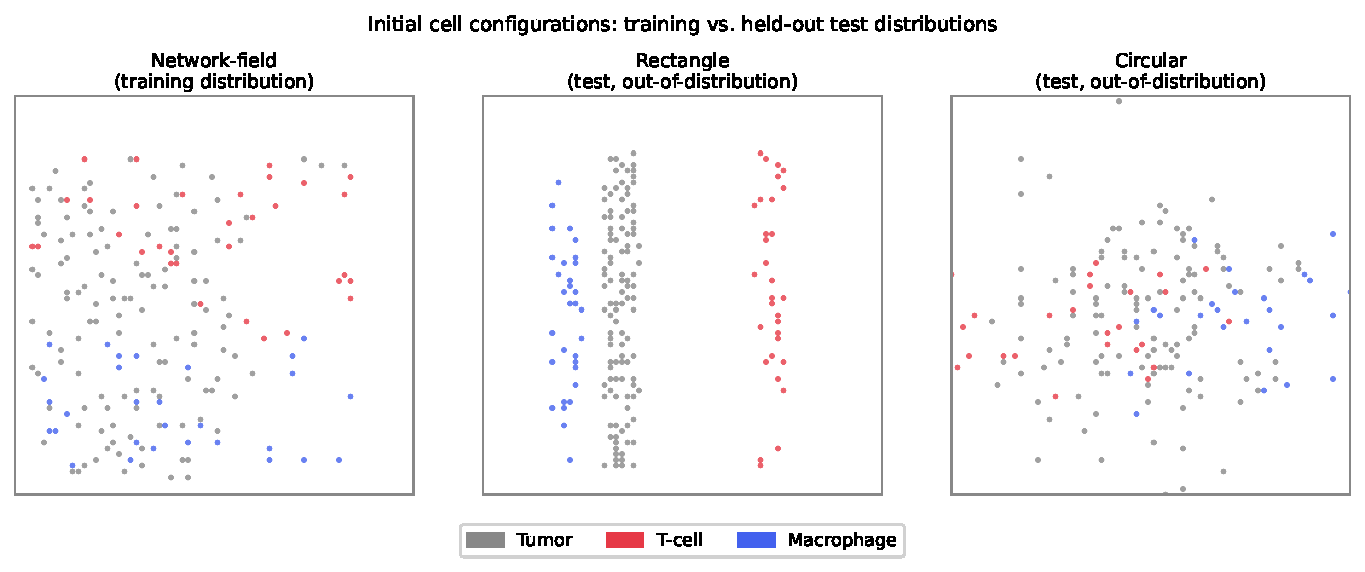
\includegraphics[width=\linewidth]{img/ic_distributions.pdf}
  \caption{Initial condition distributions.
    \emph{Left}: network-field layout (training distribution) — irregular,
    correlated clusters from a Gaussian random field.
    \emph{Centre}: circular layout (test) — tumor in an ellipse, immune
    cells in flanking clusters.
    \emph{Right}: rectangle layout (test) — each cell type confined to a
    narrow vertical strip.
    Tumor: grey $\bullet$; T-cell: red $\bullet$; macrophage: blue $\bullet$.}
  \label{fig:ic_distributions}
\end{figure}

\subsection{State space $S$: observation spaces compared}
\label{sec:obs}

In a tumor microenvironment there are different cell types and different
molecules/chemical compounds (substrates). The simulator can expose several
kinds of data: some carry explicit spatial information, others are spaceless
summaries (e.g.\ a small vector of global statistics). Because \physigym{}
can build all of these from the same underlying simulation, we use the toy model
to study how the choice of observation space affects the dynamic treatment regime
that RL learns, comparing six modes on cumulative return and on generalization to
unseen spatial configurations.

We compare six observation modes spanning a spectrum from global scalars to
full spatial images.
Let $N_c=3$ (tumor, T-cell, macrophage) and $N_s=5$ substrates.

\subsubsection*{Scalar observation spaces}

\paragraph{S1 — \Sone{} ($N_c$-dim).}
Normalised alive count per cell type:
$s_i = c_i(t)/c_{\text{init}} - 1$, $c_{\text{init}}=512$.

\paragraph{S2 — \Stwo{} ($(N_c\!+\!N_s)$-dim).}
S1 plus the domain-maximum concentration per substrate:
$s_j = \max_\mathbf{x}\,\mathrm{conc}_j(\mathbf{x},t)$.

\paragraph{S3 — \Sthree{} ($N_c + 6N_c$-dim $=21$).}
S1 plus per-type spatial statistics (6 values each):
\emph{presence flag}, centroid $(x_\mu, y_\mu)$, spread $(x_\sigma, y_\sigma)$,
and distance to domain centre — all normalised to $[0,1]$.

\paragraph{S5 — \Sfive{} ($N_c + 6N_c + 6N_s$-dim $=39$).}
S3 extended with per-substrate spatial statistics:
global mean, std, min, max, and concentration-weighted centroid $(x_c, y_c)$.

\subsubsection*{Image-based observation spaces}

The simulation domain is discretised onto a $64\!\times\!64$ pixel grid.
Cell channels: pixel $(i,j)$ receives $1/(g_xg_y)$ per cell whose position
maps to bin $(i,j)$, scaled to $[0,255]$.
Substrate channels: each bin receives the maximum concentration observed
there, then per-channel min–max normalised to $[0,255]$.

\paragraph{I1 — \Ione{} ($N_c\!\times\!64\!\times\!64$, uint8).}
One channel per cell type.

\paragraph{I2 — \Itwo{} ($(N_c\!+\!N_s)\!\times\!64\!\times\!64$, uint8).}
I1 concatenated with all five substrate concentration maps.
This is the richest observation and provides direct spatial feedback on
macrophage polarisation state via the \texttt{pro\_tumoral},
\texttt{anti\_tumoral}, and \texttt{drug\_1} channels.

\subsubsection*{Why substrate spatial maps close the feedback loop}

The indirect drug mechanism (Section~\ref{sec:model}) requires multi-step
credit assignment: the agent injects drug, macrophages polarise over several
steps, anti-tumoral gradients shift, T-cells migrate, cytokine rises, and
only then do tumor cells die.
Without substrate maps the agent observes only cell counts, and cannot
determine (i)~whether an injection reached macrophages, (ii)~whether
polarisation occurred, or (iii)~where T-cells will concentrate next.
The scalar max-concentration in S2 destroys spatial structure entirely.
Only I2's per-pixel substrate channels make the polarisation state and drug
distribution spatially legible at each step.

\subsection{Training algorithm and setup}
\label{sec:training}

To address our control objective — maximizing cancer-cell eradication while
minimizing drug administration — we employ Soft Actor-Critic
(SAC)~\citep{haarnoja2018soft}, a state-of-the-art RL algorithm for continuous
control. SAC is well suited to our setting due to its high sample efficiency,
and as a deep RL method it accommodates different observation types, such as
image-based representations, through Convolutional Neural Networks
(CNNs)~\citep{o2015introduction}. A key challenge is the computational cost of
the simulator; to alleviate this bottleneck we adopt an asynchronous parallel
training framework~\citep{mnih2016asynchronous, liu2025asynchronous}.
A GPU-resident learner updates policy and value networks asynchronously while
9 CPU-resident environment processes generate experience in parallel (see
Appendix~\ref{app:async_sac}).
On a desktop machine (32 threads, Intel i9-13900K, NVIDIA RTX 4090) with 3
threads per environment, collecting 25{,}000 steps takes $\approx6$\,min for
scalar modes and $\approx9$\,min for image modes.

\paragraph{Neural architecture.}
Scalar modes use an MLP: FC$(256)$--Mish--FC$(256)$.
Image modes use an IMPALA-style CNN~\citep{espeholt2018impala}:
\texttt{Conv}$(n_c\!\to\!32,\,8{\times}8,\,s{=}4)$--Mish--%
\texttt{Conv}$(32\!\to\!64,\,4{\times}4,\,s{=}2)$--Mish--%
\texttt{Conv}$(64\!\to\!64,\,3{\times}3,\,s{=}1)$--Mish--Flatten--%
FC$(256)$--FC$(256)$.

\paragraph{Hyperparameters.}
$5\!\times\!10^5$ total steps; replay buffer $3\!\times\!10^5$;
batch size 576; policy/Q LR $3\!\times\!10^{-4}$; $\gamma=0.99$;
$\tau=0.005$; entropy autotuning; learning starts at 5{,}000 steps;
$N_\text{env}=9$; 3--5 seeds per mode.
Test episodes (every 4 training episodes) alternate between circular and
rectangle layouts.
Metrics: \texttt{train\_return\_mean50} and \texttt{test\_return\_mean50}
(exponentially smoothed mean over 50 episodes).

% ─────────────────────────────────────────────────────────────────────────────
\section{Results}
\label{sec:results}
% ─────────────────────────────────────────────────────────────────────────────

\subsection{Aggregated performance}

Table~\ref{tab:results} summarises final performance (seeds averaged).
Figures~\ref{fig:train_curves} and~\ref{fig:test_curves} show learning curves
vs.\ cumulative environment steps with mean $\pm$ std shading across seeds.

\begin{table}[h]
  \caption{Performance at end of training ($\ge\!400$k env steps).
    Train$_\mu$/Test$_\mu$: mean smoothed return.
    Train$_\sigma$/Test$_\sigma$: std across seeds.}
  \label{tab:results}
  \centering\small
  \begin{tabular}{llccccccc}
    \toprule
    \textbf{ID} & \textbf{Mode} & \textbf{Dim} & \textbf{$n$} &
    \textbf{Train$_\mu$} & \textbf{Train$_\sigma$} &
    \textbf{Test$_\mu$}  & \textbf{Test$_\sigma$} \\
    \midrule
    I2 & img + substrates   & $8{\times}64^2$ & 5 & \textbf{+77.2} & 8.5  & \textbf{+56.5} & 10.3 \\
    I1 & img cells only     & $3{\times}64^2$ & 4 & +50.3          & 11.3 & +20.8          & 18.2 \\
    \midrule
    S3 & spatial cells      & 21              & 3 & +51.2          & 25.8 & +12.4          & 34.6 \\
    S5 & spatial cells+subs & 39              & 2 & +3.2           & 7.3  & +0.5           & 0.5  \\
    S2 & scalar cells+subs  & 8               & 4 & $-16.8$        & 38.3 & +12.3          & 27.0 \\
    S1 & scalar cells       & 3               & 4 & +5.9           & 22.0 & +17.6          & 22.5 \\
    \bottomrule
  \end{tabular}
\end{table}

\begin{figure}[h]
  \centering
  
\includegraphics[width=\linewidth]{img/train_return_mean50.pdf}
  \caption{Training return (EWMA-50, mean $\pm 1\sigma$ across seeds) vs.\
    cumulative environment steps ($\times 10^5$).
    I2 (red) separates from all other modes after $\approx\!0.5\!\times\!10^5$
    steps and widens the gap throughout training.
    Scalar modes plateau below $+35$ and exhibit high inter-seed variance
    (shaded bands).}
  \label{fig:train_curves}
\end{figure}

\begin{figure}[h]
  \centering
  
\includegraphics[width=\linewidth]{img/return_std.pdf}
  \caption{Standard deviation of return across seeds vs.\ environment steps:
    training (left) and test (right).
    Image modes (I1, I2) maintain consistently lower std than scalar modes
    throughout training.
    I2's train std (${\approx}8.5$) is 3--4$\times$ lower than S2's (${\approx}38.3$),
    confirming that spatial substrate representations produce more robust
    learning dynamics across random initialisations.}
  \label{fig:std_curves}
\end{figure}

\begin{figure}[h]
  \centering
  
\includegraphics[width=\linewidth]{img/test_return_mean50.pdf}
  \caption{Test return (mean $\pm 1\sigma$ across seeds, EWMA-50) vs.\
    cumulative environment steps.
    Test episodes alternate between circular and rectangle held-out layouts.
    I2 consistently climbs throughout training; I1 and scalar modes show
    little improvement and high variance, confirming that substrate spatial
    information is required for generalisation to OOD layouts.}
  \label{fig:test_curves}
\end{figure}

\subsection{Key findings}

\paragraph{Substrate channels are decisive.}
Adding substrate maps to the cell-only image (I1$\to$I2) raises training
return by $+27$ and test return by $+36$ points — the largest single
improvement in the comparison.
Adding substrate \emph{scalars} (S1$\to$S2) gives $-22$ points on training
return and raises seed variance to $\sigma=38.3$, confirming that spatially
aggregated substrate values are not only insufficient but harmful.

\paragraph{More scalar features does not help.}
Scalar complexity increases S1(3)$\to$S2(8)$\to$S3(21)$\to$S5(39), but
train mean follows $+5.9\to-16.8\to+51.2\to+3.2$.
S3's centroid statistics help; adding substrate spatial statistics (S5) hurts,
likely because the 39-dim space is harder to optimise in 500k steps.

\paragraph{Seed robustness.}
Image modes show 3--4$\times$ lower seed variance than scalar modes
(Table~\ref{tab:results}, Figure~\ref{fig:train_curves} right).
I2's train std is $8.5$ vs.\ S2's $38.3$.
The CNN inductive bias (spatial locality, translation equivariance) aligns
with the TME's physical structure and consistently guides optimisation
regardless of random initialisation.

\subsection{Generalisation to held-out layouts}

\begin{table}[h]
  \caption{Test return by held-out layout (seeds averaged).}
  \label{tab:layouts}
  \centering\small
  \begin{tabular}{lrrr}
    \toprule
    \textbf{Mode} & \textbf{Test avg} & \textbf{Rectangle} & \textbf{Circular} \\
    \midrule
    I2 & \textbf{+56.5} & +44.5 & \textbf{+97.9} \\
    I1 & +20.8          & $-0.6$ & +5.0 \\
    S3 & +12.4          & \textbf{+112.7}$^\dagger$ & +16.3 \\
    S5 & +0.5           & +85.1 & $-37.6$ \\
    S2 & +12.3          & +40.2 & $-47.7$ \\
    S1 & +17.6          & $-7.7$ & $-20.5$ \\
    \bottomrule
  \end{tabular}
  {\small $^\dagger$Driven by a single seed (seed 64: $+223$); seed 1 collapses to $-28.9$.}
\end{table}

I2 achieves the highest \emph{average} test return and the highest circular
return ($+97.9$).
I1 fails on both OOD layouts (near zero or negative), confirming that
cell-image policies overfit to the training network-field geometry without
substrate feedback.
The S3 rectangle outlier is a single seed; its circular return is $+16.3$,
illustrating the inconsistency of scalar-mode generalisation.

\subsection{Episode analysis}

We compare two matched test episodes at different training checkpoints:
run\_000143 (seed~64, early-to-mid training) and run\_000147 (seed~128,
later training).
All three agents start from the same initial conditions in each case.

\begin{figure}[h]
  \centering
  
\includegraphics[width=\linewidth]{img/fig_episode_comparison.pdf}
  \caption{\textbf{Episode run\_000143, seed~64.}
    Cumulative return (top), cumulative drug (middle), per-step dose (bottom).
    I2: near-eradication (4 tumor cells, $+175$ return, 35.4 total dose).
    S3: partial control (14 cells, $+106$ return, 31.1 total dose).
    I1: failure (112 cells, $-7.4$ return, only 12.2 total dose).
    Despite similar total drug between I2 and S3, only I2 eradicates the
    tumor: spatial substrate maps enable precise drug placement that converts
    dose into effective macrophage repolarisation.}
  \label{fig:episode}
\end{figure}

\begin{figure}[h]
  \centering
  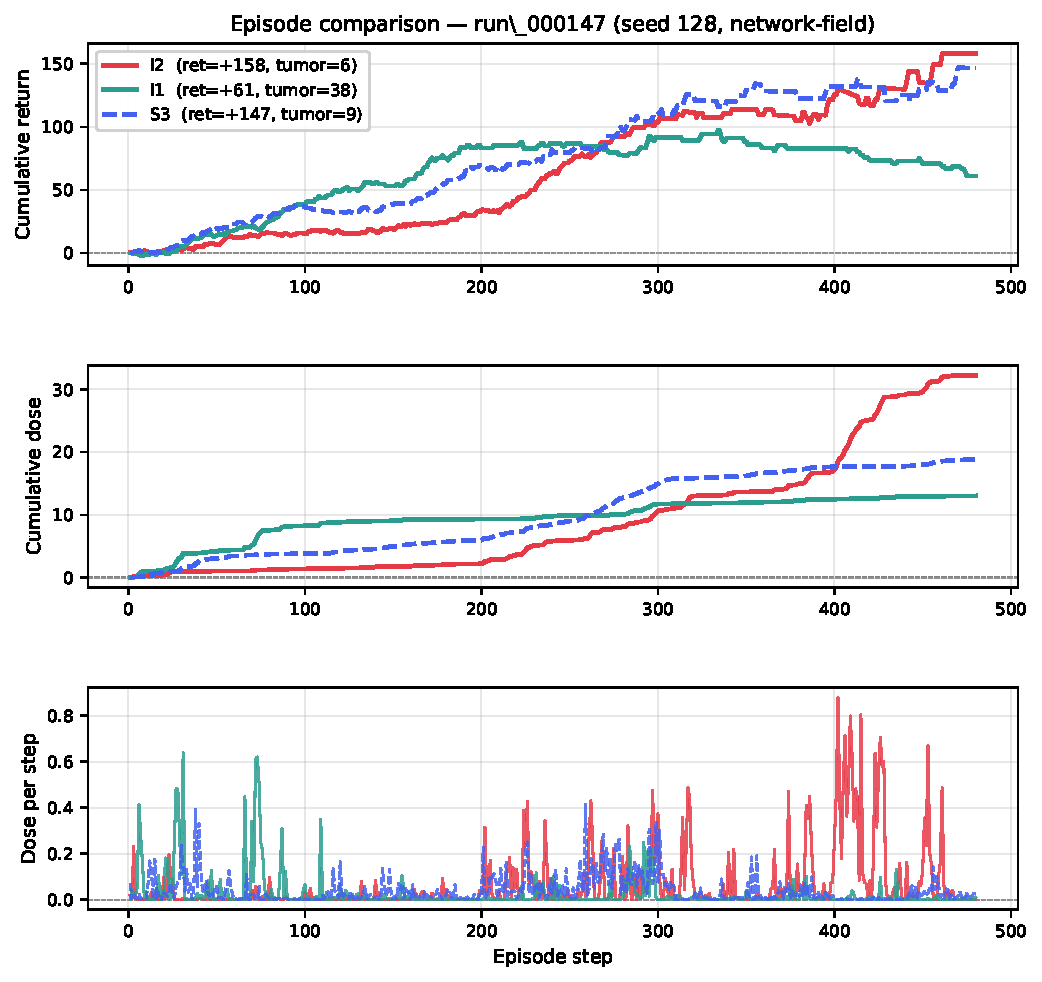
\includegraphics[width=\linewidth]{img/fig_episode_comparison_2.pdf}
  \caption{\textbf{Episode run\_000147, seed~128.}
    A harder episode: no agent achieves eradication.
    I2: $+158$ return (6 tumor cells, 32.2 total dose).
    I1: $+61$ return (38 cells, 13.0 total dose).
    S3: $+147$ return (9 cells, 18.9 total dose).
    Comparing with run\_000143: when near-eradication is achievable I2
    dominates; when the tumor is more resilient all agents struggle with
    rebound, but I2 maintains the best final tumor count.
    I1 again under-medicates ($13.0$ vs.\ $32.2$ for I2).}
  \label{fig:episode2}
\end{figure}

\paragraph{Failure modes.}
Across both episodes two failure modes are consistent:
(i)~\textbf{I1 under-medicates}: without substrate channels the agent
cannot determine whether injections reached macrophages, converging to a
conservative low-dose policy (12--13 total dose vs.\ 32--35 for I2).
(ii)~\textbf{S3 partially controls but cannot finish}: centroid features
enable rough spatial targeting for early suppression, but without knowing
where \texttt{pro\_tumoral} is suppressing T-cell infiltration, the agent
cannot commit to the final targeted burst needed for eradication.

% ─────────────────────────────────────────────────────────────────────────────
\section{Discussion}
% ─────────────────────────────────────────────────────────────────────────────

The central outcome of this work is \physigym{} itself: a framework that lets
RL agents control a full agent-based TME through a standardised interface,
without recompilation, and with arbitrary observation and action spaces. The
toy-model case study shows the framework end-to-end — an agent learns a spatial
drug-delivery policy that steers the microenvironment toward an anti-tumoral
state and, in the best episodes, eradicates the tumor.

The toy model also yields a clear result on observation spaces. Spatially
explicit (image) observations consistently outperform global scalar summaries,
and substrate spatial maps are the most informative of all: the CNN in I2 can
compute cross-channel co-localisation statistics (e.g.\ whether \texttt{drug\_1}
and macrophages overlap at the same location) that would require explicit
engineered features in any scalar representation, while the scalar
max-concentration in S2 discards spatial structure entirely. The same ordering
holds for generalization to held-out layouts: I2 transfers because substrate
gradients are spatially informative regardless of initial geometry, whereas
scalar modes encoding absolute centroid positions tend to overfit to the
training distribution.

We emphasise that this is an application-level observation on a deliberately
simplified model, not a universal claim about biological control. In more
complex or realistic models — or with different reward designs, action spaces,
or RL algorithms — the relative value of cell versus substrate, and scalar
versus image, may differ. \physigym{} is precisely the tool that makes such
questions answerable in a reproducible way.

\paragraph{Limitations.}
The toy model is intentionally small (63\,$\mu$m, 2D) and cheap to simulate.
Scaling to 3D or larger domains will increase the cost of image observations.
All experiments use a single RL algorithm (SAC); alternative algorithms or
model-based methods may interact differently with observation spaces.
Relational and K-means scalar modes, which may partially close the gap with I2
at lower computational cost, are left to future work.

% ─────────────────────────────────────────────────────────────────────────────
\section{Conclusion}
% ─────────────────────────────────────────────────────────────────────────────

We presented \physigym{}, an open-source framework that bridges the
\physicell{} ABM with Gymnasium RL, enabling direct policy learning in
spatially explicit biological simulations.
Using a TME model with an indirect drug mechanism, we showed that full
spatial substrate images are the critical state representation: they raise
training return by $+71$ points and test return by $+39$ points over pure
scalar baselines.
The mechanism is causal — substrate maps close the feedback loop between drug
injection and macrophage repolarisation that is invisible to all scalar modes.
\physigym{} provides the infrastructure to study such questions in a
principled, reproducible manner, and we anticipate it will serve as a
testbed for both computational biology and RL communities.

% ─────────────────────────────────────────────────────────────────────────────
\begin{ack}
A.B., V.P., and E.R.\ acknowledge funding from Region Occitanie and INSERM,
Projet Emergence REACT.
E.B.\ received support from a Chateaubriand Fellowship of the Office for
Science \& Technology of the Embassy of France in the United States.
This study was partially supported through grant EUR CARe N°ANR-18-EURE-0003
and an Eiffel Excellence doctoral fellowship to M.H.
This research was also supported in part by Lilly Endowment, Inc., through its
support for the Indiana University Pervasive Technology Institute.
No competing interests are declared.
\end{ack}

% ─────────────────────────────────────────────────────────────────────────────
\bibliographystyle{abbrvnat}
\bibliography{reference}

% ─────────────────────────────────────────────────────────────────────────────
\appendix

\section{Generation of Initial Conditions}
\label{app:ic}

White Gaussian noise $\eta(\mathbf{x})\sim\mathcal{N}(0,1)$ is convolved
with a Gaussian kernel $G_\sigma$ ($\sigma=\ell_c/\sqrt{2}$,
$\ell_c=45$\,µm) to produce a correlated field $F$.
An additional local noise component $\tilde\xi$ filtered at width
$\ell_c/3$ is added with small weight $\alpha$ to introduce local
heterogeneity.
The field is normalised to $[0,1]$ and cells are sampled from positions
with $\hat{F}>0.55$, with probability proportional to $\hat{F}$.

For the circular test layout, tumor cells are placed in a random ellipse
(semi-axes $r_1 \in [0.1,0.4]$, $r_2 \in [0.1,0.4]$ of the half-domain)
centred on the domain, and immune cells in two flanking ellipses at 20\%
and 80\% of the $x$-axis (shuffled between T-cells and macrophages).
For the rectangle layout, each cell type is placed uniformly in a vertical
strip of width 10\% of the $x$-axis, with non-overlapping strip positions
sampled from $[0.1,0.2]$, $[0.3,0.5]$, $[0.6,0.8]$ (shuffled across types).
See \texttt{init\_conds\_v3.py} for the full implementation.

\section{Asynchronous SAC}
\label{app:async_sac}

\begin{algorithm}[H]
\caption{Asynchronous SAC with Parallel Environments~\citep{liu2025asynchronous}}
\label{alg:async_sac}
\begin{algorithmic}[1]
\Require Config $d_\text{arg}$, buffer size $|\mathcal{B}|$, LRs, $\gamma$, $\tau$
\State Init shared queues \texttt{actor\_queue}, \texttt{sample\_queue};
       stop signal \texttt{stop\_event}
\State \textbf{Actor Process (CPU):} init $N_\text{env}=9$ envs, local $\pi_{\theta_a}$
\While{not \texttt{stop\_event}}
  \State Receive $\theta$ from \texttt{actor\_queue} if available
  \State Act: random if $t\!<\!T_\text{start}$, else $\pi_{\theta_a}$
  \State Step envs; push $(s,a,r,s',d)$ to \texttt{sample\_queue}
\EndWhile
\State \textbf{Learner Process (GPU):} init $\pi_\theta$, $Q_{\phi_{1,2}}$, targets, $\mathcal{D}$
\While{total samples $< T$}
  \State Drain \texttt{sample\_queue} into $\mathcal{D}$
  \For{$N_\text{loops}$ gradient steps}
    \State Sample minibatch; compute SAC target $y$; update $Q$, $\pi$, $\alpha$;
           soft-update targets
  \EndFor
  \State Push updated $\theta$ to \texttt{actor\_queue}
\EndWhile
\end{algorithmic}
\end{algorithm}

\section{Hyperparameters}
\label{app:hyperparams}

\begin{table}[h]
  \centering\small
  \caption{SAC hyperparameters (TME v2 experiments).}
  \label{tab:hyperparams}
  \begin{tabular}{lll}
    \toprule
    \textbf{Parameter} & \textbf{Symbol} & \textbf{Value} \\
    \midrule
    Total training steps & $T$              & $5\!\times\!10^5$ \\
    Replay buffer size   & $|\mathcal{B}|$  & $3\!\times\!10^5$ \\
    Batch size           & $B$              & 576 \\
    Warm-up steps        & $T_\text{start}$ & 5{,}000 \\
    Policy / critic LR   & $\eta_\pi,\eta_Q$& $3\!\times\!10^{-4}$ \\
    Discount factor      & $\gamma$         & 0.99 \\
    Target smoothing     & $\tau$           & 0.005 \\
    Entropy autotuning   & --               & enabled \\
    Parallel envs        & $N_\text{env}$   & 9 \\
    Update loops / step  & $N_\text{loops}$ & 3 \\
    Test frequency       & --               & every 4 episodes \\
    \bottomrule
  \end{tabular}
\end{table}

\section{Per-Seed Results}
\label{app:per_seed}

\begin{table}[h]
  \centering\small
  \caption{Per-seed results. Rect/Circ: mean return on rectangle/circular test layout.}
  \label{tab:per_seed}
  \begin{tabular}{llccccc}
    \toprule
    \textbf{Mode} & \textbf{Seed} & \textbf{Steps} & \textbf{Train50} &
    \textbf{Test50} & \textbf{Rect} & \textbf{Circ} \\
    \midrule
    I2 & 1   & 499,356 & +78.0 & +58.2 & +4.4    & +106.7 \\
    I2 & 32  & 529,501 & +79.7 & +69.9 & +4.9    & +61.4  \\
    I2 & 64  & 410,875 & +86.9 & +47.7 & +109.6  & +33.7  \\
    I2 & 64  & 499,977 & +64.3 & +42.3 & +47.3   & +128.9 \\
    I2 & 128 & 499,914 & +77.1 & +64.5 & +56.1   & +158.8 \\
    \midrule
    I1 & 1   & 499,884 & +39.8 & +22.4 & $-28.7$ & $-28.1$ \\
    I1 & 32  & 526,602 & +42.4 & +27.8 & $-17.4$ & $-43.9$ \\
    I1 & 64  & 499,769 & +51.3 & +14.5 & $-0.5$  & $-2.8$  \\
    I1 & 128 & 499,632 & +67.5 & +18.3 & +44.2   & +94.8   \\
    \midrule
    S3 & 1   & 499,976 & +16.7 & $-28.9$ & +32.2   & $-81.3$ \\
    S3 & 64  & 499,996 & +59.8 & +27.3 & +223.1  & +91.1   \\
    S3 & 128 & 499,990 & +77.1 & +38.8 & +82.9   & +39.2   \\
    \midrule
    S5 & 1   & 499,979 & +10.4 & +1.2  & +6.0    & $-67.5$ \\
    S5 & 64  & 499,979 & $-4.1$& $-0.1$& +164.2  & $-7.6$  \\
    \midrule
    S2 & 1   & 499,939 & +1.7  & +26.8 & +144.6  & $-0.6$  \\
    S2 & 32  & 528,409 & $-79.2$& $-24.6$& $-4.8$ & $-90.8$ \\
    S2 & 64  & 499,942 & +25.3 & +18.8 & +8.0    & $-44.4$ \\
    S2 & 128 & 499,959 & $-15.1$& +28.1 & +12.9  & $-54.8$ \\
    \midrule
    S1 & 1   & 499,925 & +37.2 & +24.0 & $-1.5$  & $-21.8$ \\
    S1 & 32  & 527,895 & +6.2  & +23.3 & +30.3   & +46.7   \\
    S1 & 64  & 499,988 & $-20.3$& +6.9 & $-52.6$ & $-33.1$ \\
    S1 & 128 & 499,938 & +0.4  & +16.3 & $-6.9$  & $-74.0$ \\
    \bottomrule
  \end{tabular}
\end{table}

\end{document}
